\begin{figure}
\captionsetup[sub]{font=scriptsize}
\begin{subfigure}[b]{.19\linewidth}
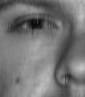
\includegraphics[width = \linewidth]{DN_yale/yale_03_1_cauchy_st_fsim} 
\caption{Cauchy ST}
\end{subfigure}\hfill
\begin{subfigure}[b]{.19\linewidth}
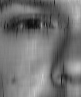
\includegraphics[width = \linewidth]{DN_yale/yale_03_1_welsh_st_fsim} 
\caption{Welsh ST}
\end{subfigure}\hfill
\begin{subfigure}[b]{.19\linewidth}
    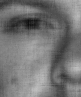
\includegraphics[width = \linewidth]{DN_yale/yale_03_1_cvpr2016_tnn_fsim}
    \caption{TRPCA '16}
\end{subfigure}\hfill
\begin{subfigure}[b]{.19\linewidth}
    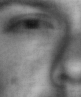
\includegraphics[width = \linewidth]{DN_yale/yale_03_1_horpca_s_fsim} 
    \caption{HORPCA-S}
\end{subfigure}\hfill
\begin{subfigure}[b]{.19\linewidth}
    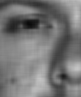
\includegraphics[width = \linewidth]{DN_yale/yale_03_1_nctrpca_fsim} 
    \caption{NCTRPCA}
\end{subfigure}\hfill
\begin{subfigure}[b]{.19\linewidth}
    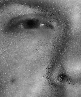
\includegraphics[width = \linewidth]{DN_yale/yale_03_1_rnndl_fsim} 
    \caption{RNNDL}
\end{subfigure}\hfill
\begin{subfigure}[b]{.19\linewidth}
    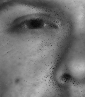
\includegraphics[width = \linewidth]{DN_yale/yale_03_1_rpca_fsim} 
    \caption{RPCA}
\end{subfigure}\hfill
\begin{subfigure}[b]{.19\linewidth}
    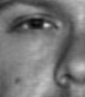
\includegraphics[width = \linewidth]{DN_yale/yale_03_1_rpca2d_l1_fsim}
    \caption{KDRSDL}
\end{subfigure}
\begin{subfigure}[b]{.19\linewidth}
    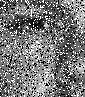
\includegraphics[width = \linewidth]{Ref/yale_1_03_original}
    \caption{Noisy}
\end{subfigure}
\begin{subfigure}[b]{.19\linewidth}
    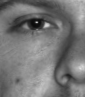
\includegraphics[width = \linewidth]{Ref/yale_1_original} 
    \caption{Original}
\end{subfigure}
\caption{Results on the Yale benchmark with 30\% noise. TRPCA '14 removed.}
\label{fig:visual_yale_30}
\end{figure}

%\begin{subfigure}[b]{.19\linewidth}
%\includegraphics[width = \linewidth]{DN_yale/yale_03_1_cvpr2014_tsvd_fsim} 
%\caption{TRPCA '14}
%\end{subfigure}\hfill